\section{Benutzungsoberfläche}


\subsection{Startfenster}

\begin{figure}[!hp] 
  \centering
     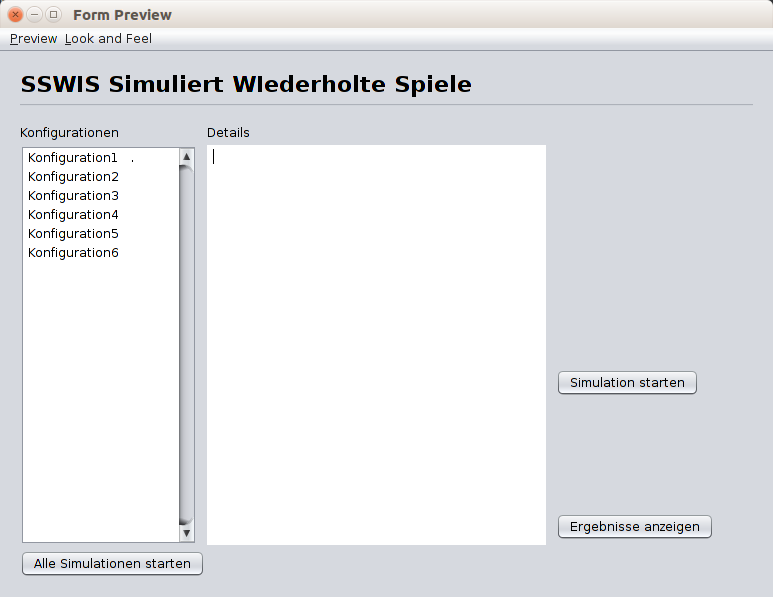
\includegraphics[width=0.9\textwidth]{GUI_Entwurf/Startfenster.png}
  \caption{Hauptfenster}
  \label{fig:Bild1}
\end{figure}

\begin{description}


\item[1. Menüleiste] Enthält den Menüpunkt:
	\begin{itemize}
		\item{Neu}
		\begin{itemize}
			\item{Stufenspiel}
			\item{Kombinierte Strategie}
			\item{Initialisierung}
			\item{Konfiguration}
		\end{itemize}
		\item{Verwalten}
		\begin{itemize}
			\item{Stufenspiele}
			\item{Kombinierte Strategien}
			\item{Initialisierungen}
			\item{Konfigurationen}
			\item{Ergebnisse}
		\end{itemize}
	\end{itemize}

\item[2. Liste der Konfigurationen] Alle erstellten oder gespeicherten Konfigurationen, werden hier angezeigt. Einzelne Konfigurationen einer Mehrfachkonfiguration werden als Unterpunkte dieser dargestellt. Es kann genau eine Konfiguration oder Mehrfachkonfiguration ausgewählt werden. In Tooltips werden Details zu den Konfigurationen angezeigt.

\item[3. Button - Simulation starten] Ist eine Konfiguration in der obigen Liste ausgewählt, ist dieser Button aktiviert. Nach dem Betätigen wird in einem Pop-Up-Fenster die Anzahl der Wiederholungen abgefragt. Danach werden die Simulation mit der ausgewählten Konfiguration gestartet.

\item[4. Button - Ergebnisse speichern] Wurde die in der Liste ausgewählte Konfiguration bereits simuliert, ist dieser Button aktiviert. Er speichert die Ergebnissen, der zuletzt durchgeführten Simulationen.

\item[5. Button - Ergebnisse anzeigen] Wurde die in der Liste ausgewählte Konfiguration bereits simuliert, ist dieser Button aktiviert. Er öffnet das Ergebnisfenster mit den Ergebnissen, der zuletzt durchgeführten Simulationen.



\end{description}

\pagebreak

\subsection{Stufenspiele Verwalten}

\begin{figure}[!hp] 
  \centering
     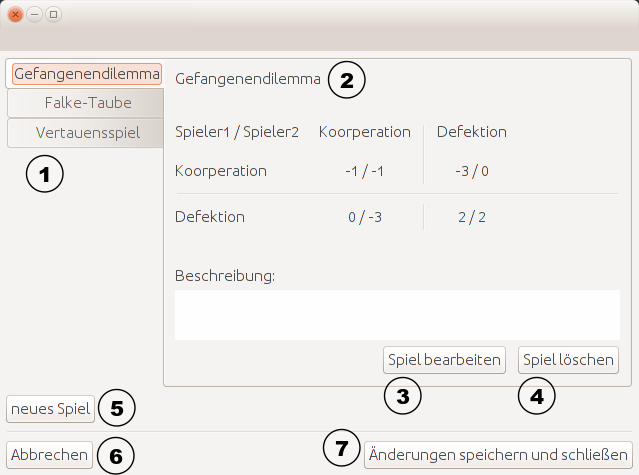
\includegraphics[width=1.1\textwidth]{GUI_Entwurf/SpieleVerwalten.png}
  \caption{Stufenspiel Verwaltung}
  \label{fig:Bild1}
\end{figure}

\begin{description}

\item[1. Tabfenster] Enthält alle zuvor gespeicherten und voreingestellten Stufenspiele als Tab.

\item[2. Tab] Im Tab werden alle Details, des jeweiligen Stufenspiels angezeigt: Name, Tabelle der Auszahlungen und Beschreibung.

\item[3. Button - Spiel bearbeiten] Öffnet das Fenster zum Bearbeiten von Stufenspielen.

\item[4. Button - Spiel löschen] Das Stufenspiel, des gewählten Tabs, wird gelöscht.

\item[5. Button - neues Spiel] Es öffnet sich ein neues Dialogfenster, wo der Name des Spiels eingegeben werden kann und der Nutzer wird anschließend zum Fenster zum Bearbeiten von Stufenspielen weitergeleitet.

\item[6. Abbrechen] Alle zuvor vorgenommen Änderungen inklusive das Erstellen neuer Spiele werden verworfen und die Spiele Verwaltung schließt sich.

\item[7. Änderungen speichern und schließen] Alle zuvor vorgenommen Änderungen werden gespeichert und die Spiele Verwaltung schließt sich.

\end{description}



\subsection{Stufenspiele Bearbeiten}

In dem Fenster zum Bearbeiten von Stufenspielen, können die einzelnen Auszahlungen und eine Beschreibung zu dem Spiel in entsprechenden Textfeldern eingegeben werden. Die Auszahlungen sind wie in der Verwaltung in einer Tabelle angeordnet. Der Name des Spiels wird angezeigt.
Durch eine Button \textit{speichern} können die Eingaben gespeichert und das Fenster anschließend geschlossen werden.  Durch einen weiteren Button \textit{abbrechen} werden die Änderungen verworfen und das Fenster wird ebenfalls  geschlossen.  

\pagebreak

\subsection{Kombinierte Strategien Verwalten}


\begin{figure}[!hp]
  \centering
     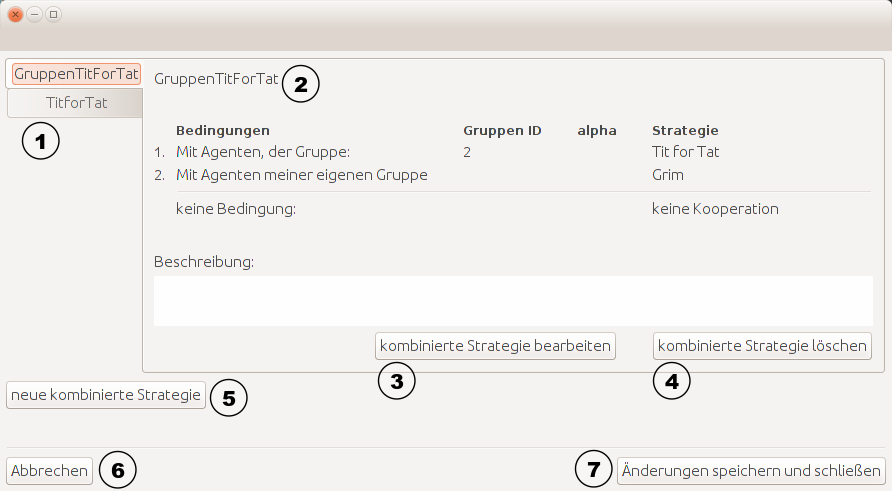
\includegraphics[width=1.15\textwidth]{GUI_Entwurf/StrategienVerwalten.png}
  \caption{Kombinierte Strategien Verwaltung}
  \label{fig:Bild1}
\end{figure}

\begin{description}

\item[1. Tabfenster] Enthält alle zuvor gespeicherten kombinierte Strategien als Tab.

\item[2. Tab] Im Tab werden alle Details, der jeweiligen kombinierten Strategie angezeigt: Name, Tabelle der Bedingungen und Strategien, und die Beschreibung.

\item[3. Button - kombinierte Strategie bearbeiten] Öffnet das Fenster zum Bearbeiten von kombinierten Strategie.

\item[4. Button - kombinierte Strategie löschen] Die kombinierte Strategie, des gewählten Tabs, wird gelöscht.

\item[5. Button - neue kombinierte Strategie] Es öffnet sich ein neues Dialogfenster, wo der Name der kombinierte Strategie eingegeben werden kann und der Nutzer wird anschließend zum Fenster zum Bearbeiten von kombinierten Strategien weitergeleitet.

\item[6. Abbrechen] Alle zuvor vorgenommen Änderungen inklusive das Erstellen neuer kombinierter Strategien werden verworfen und die kombinierte Strategien Verwaltung schließt sich.

\item[7. Änderungen speichern und schließen] Alle zuvor vorgenommen Änderungen werden gespeichert und die kombinierte Strategien Verwaltung schließt sich.

\end{description}


\subsection{Kombinierte Strategien Bearbeiten}

In dem Fenster zum Bearbeiten von kombinierten Strategien, können die einzelnen Bedingungen und zugehörige Strategien in Dropdown-Menüs gewählt werden. Die Bedingungen sind wie in der Verwaltung in einer Tabelle angeordnet. Der Name der kombinierte Strategie wird angezeigt. Eine Beschreibung kann in einem Textfeld angegeben werden.
Durch einen Button \textit{speichern} können die Eingaben gespeichert und das Fenster anschließend geschlossen werden. Durch einen weiteren Button \textit{abbrechen} werden die Änderungen verworfen und das Fenster wird ebenfalls  geschlossen.  

\pagebreak

\subsection{Initailisierung Verwalten}

Die Verwaltung für Initialisierungen ist analog zu der von Stufenspielen und kombinierten Strategien aufgebaut. In den einzelen Tabs, werden Details zur jeweiligen Initialisierung angezeigt: Name, Anzahl der Agenten, Gruppen mit: ID, Name, Agenten, Strategien-Verteilung, Startkapital-Verteilung.


\subsection{Initialisierung Bearbeiten}

\begin{figure}[!hp] 
  \centering
     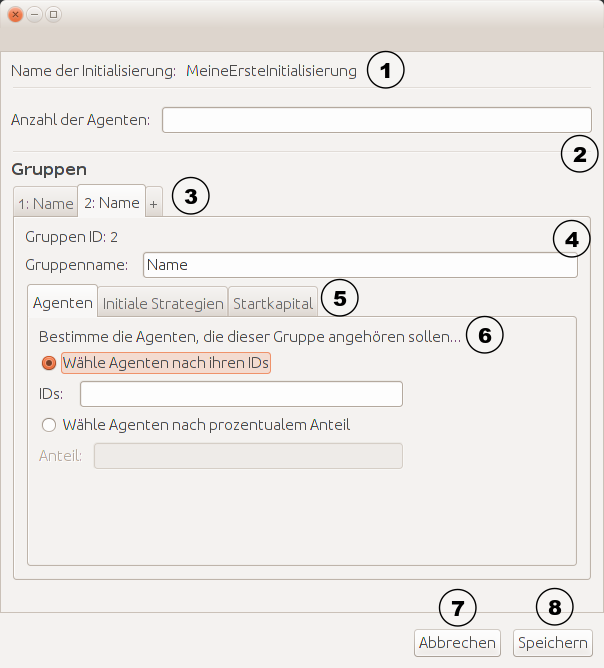
\includegraphics[width=1.0\textwidth]{GUI_Entwurf/InitialisierungBearbeiten1.png}
  \caption{Initialisierung}
  \label{fig:Bild1}
\end{figure}


\begin{description}

\item[1. Name] Name der Initialisierung.

\item[2. Anzahl der Agenten] Anzahl der Agenten soll hier angegeben werden. Es können auch variable Werte der Form \textit{Startwert - Endwert - Schrittweite} eingegeben werden.

\item[3. Tabfenster - Gruppen] Zu jeder Gruppe gibt es ein Tab. Durch wählen des '+' Tabs wird eine weitere Gruppe hinzugefügt.

\item[4. Gruppen - ID und Name] Die Gruppen ID wird automatisch vergeben. Der Gruppen Name soll hier angegeben werden.

\item[5. Tabfenster - Spezifikation] Es kann zwischen den Tabs 'Agenten', 'Initiale Strategien' und 'Startkapital' gewählt werden.   

\item[6. Bestimme Agenten, die dieser Gruppe angehören sollen] Die Agenten sollen entweder nach einem prozentualen Anteil aller Agenten oder nach ihren IDs gewählt werden. Es können auch variable Werte der Form \textit{Startwert - Endwert - Schrittweite} eingegeben werden.

\item[7. Abbrechen] Alle Änderungen werden verworfen und das Fenster wird geschlossen.

\item[8. Speichern] Alle Änderungen werden gespeichert und das Fenster wird geschlossen.

\end{description}
\pagebreak



\begin{figure}[!hp] 
  \centering
     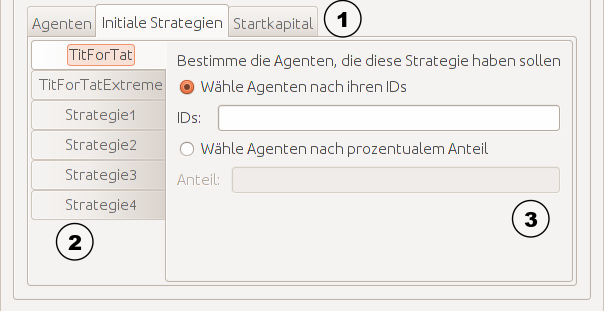
\includegraphics[width=1.0\textwidth]{GUI_Entwurf/InitialisierungBearbeiten2.png}
  \caption{Tab - Initiale Strategien}
  \label{fig:Bild1}
\end{figure}

\begin{description}

\item[1. Tabfenster - Spezifikation] Es kann zwischen den Tabs 'Agenten', 'Initiale Strategien' und 'Startkapital' gewählt werden.  

\item[2. Tabfenster - Initiale Strategien] Alle erstellten kombinierten Strategien sind in Tabs aufgelistet. 

\item[3. Tab] In jedem Tab können die Agenten, mit der jeweiligen kombinierten Strategie gewählt werden. Es kann nur aus Agenten innerhalb der Gruppe gewählt werden. Die Agenten sollen entweder nach einem prozentualen Anteil aller Agenten der Gruppe oder nach ihren IDs gewählt werden. Es können auch variable Werte der Form \textit{Startwert - Endwert - Schrittweite} eingegeben werden.

\end{description}


\begin{figure}[!hp] 
  \centering
     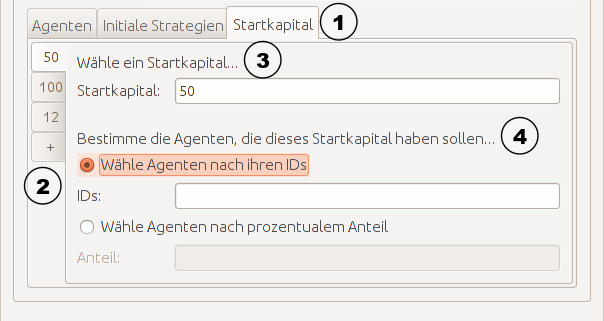
\includegraphics[width=1.0\textwidth]{GUI_Entwurf/InitialisierungBearbeiten3.png}
  \caption{Tab - Startkapital}
  \label{fig:Bild1}
\end{figure}

\begin{description}

\item[1. Tabfenster - Spezifikation] Es kann zwischen den Tabs 'Agenten', 'Initiale Strategien' und 'Startkapital' gewählt werden.  

\item[2. Tabfenster - Startkapital] Hier können mehrere Werte für ein Startkapital festgelegt werden. Mit Wählen des '+' Tabs wird ein weiterer Wert hinzugefügt.

\item[3. Tab] In jedem Tab können die Agenten, mit dem jeweiligen Startkapital gewählt werden. Es kann nur aus Agenten innerhalb der Gruppe gewählt werden. Die Agenten sollen entweder nach einem prozentualen Anteil aller Agenten der Gruppe oder nach ihren IDs gewählt werden. Es können auch variable Werte der Form \textit{Startwert - Endwert - Schrittweite} eingegeben werden.

\end{description}

\pagebreak

\subsection{Konfigurationen Verwalten}

Die Verwaltung für Konfigurationen ist analog zu der von Stufenspielen und kombinierten Strategien aufgebaut. In den einzelen Tabs, werden Details zur jeweiligen Konfiguration angezeigt.

\subsection{Konfigurationen Bearbeiten}

\begin{figure}[!hp] 
  \centering
     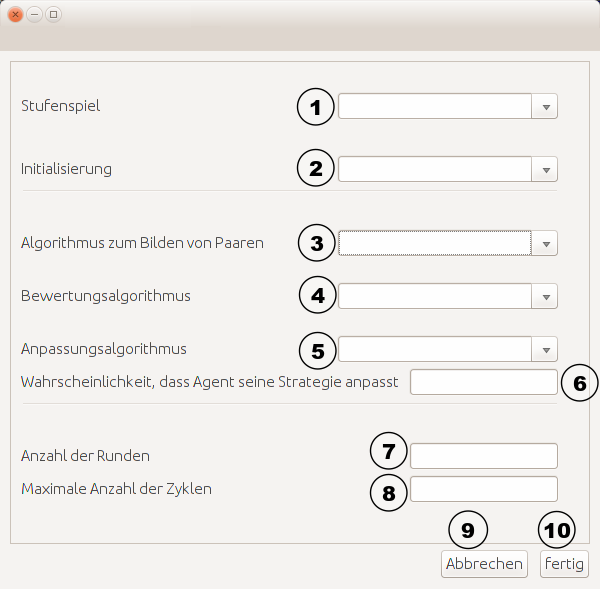
\includegraphics[width=1.0\textwidth]{GUI_Entwurf/KonfigurationBearbeiten.png}
  \caption{Konfiguration Bearbeiten}
  \label{fig:Bild2}
\end{figure}



\begin{description}

\item[1. Stufenspiel] Hier kann eines von den gespeicherten und voreingestellten Stufenspielen ausgewählt werden.

\item[2. Initialisierung] Hier kann eine zuvor gespeicherte Initialisierung ausgewählt werden. 

\item[3. Algorithmus zum Bilden von Paaren] Hier soll ein Algorithmus zum Bilden von Paaren gewählt werden. 

\item[4. Bewertungsalgorithmus] Hier soll ein Algorithmus zum Bilden von Paaren gewählt werden.

\item[5. Anpassungsalgorithmus] Hier soll ein Algorithmus zum Bilden von Paaren gewählt werden.

\item[6. Wahrscheinlichkeit für Strategieanpassung] Hier soll die Wahrscheinlichkeit für Strategieanpassung angegeben werden. Es können auch variable Werte der Form \textit{Startwert - Endwert - Schrittweite} eingegeben werden.

\item[7. Anzahl der Runden] Hier soll die Anzahl der Runden angegeben werden. Es können auch variable Werte der Form \textit{Startwert - Endwert - Schrittweite} eingegeben werden.

\item[8. Maximale Anzahl der Zyklen] Hier soll die maximale Anzahl der Zyklen angegeben werden. Es können auch variable Werte der Form \textit{Startwert - Endwert - Schrittweite} eingegeben werden.

\item[9. fertig] Das Fenster wird geschlossen und die durch die Parameter bestimmten Konfigurationen werden auf die Startseite geladen.

\item[10. Abbrechen] Alle Eingaben werden verworfen und das Fenster wird geschlossen.


\end{description}

\pagebreak



\subsection{Ergebnisse Anzeigen}

\begin{figure}[!hp] 
  \centering
     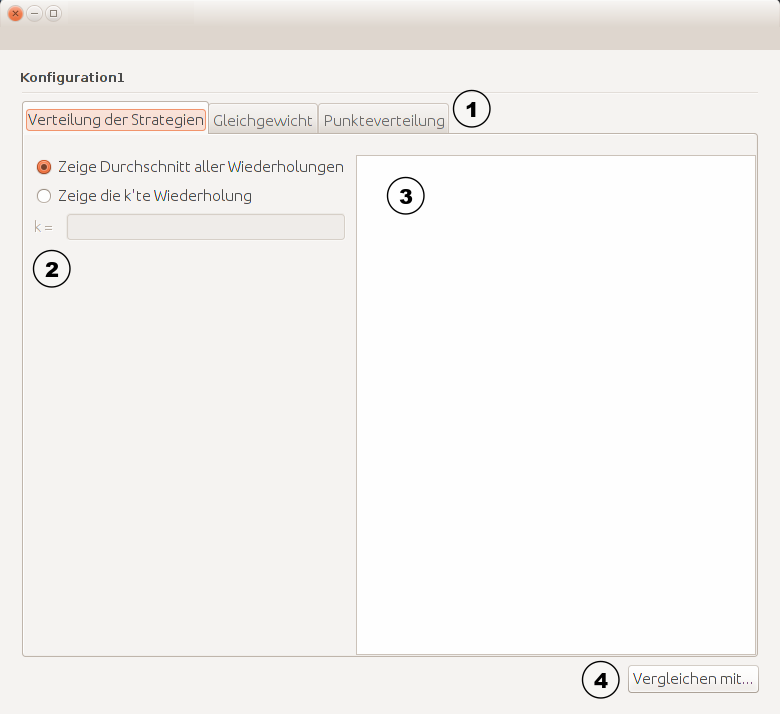
\includegraphics[width=1.1\textwidth]{GUI_Entwurf/EinfacheErgebnisse.png}
  \caption{Ergebnisfenster}
  \label{fig:Bild7}
\end{figure}

\begin{description}

\item[1. Tabfenster] In den Tabs kann zwischen verschiedenen Ergebnissansichten gewechselt werden.

\item[2. Wiederholung] In jedem Tab kann gewählt werden, ob die Ergebnisse als Durchschnitt aller Wiederholungen oder, ob die Ergebnisse einer bestimmten Wiederholung angezeigt werden sollen.

\item[3. Ergebnisfenster] In diesem Fenster werden die Ergebnisse und zugehörige Diagramme angezeigt.

\item[5. Vergleichen mit...] Öffnet das Vergleichfenster.

\end{description}


\begin{figure}[!hp] 
  \centering
     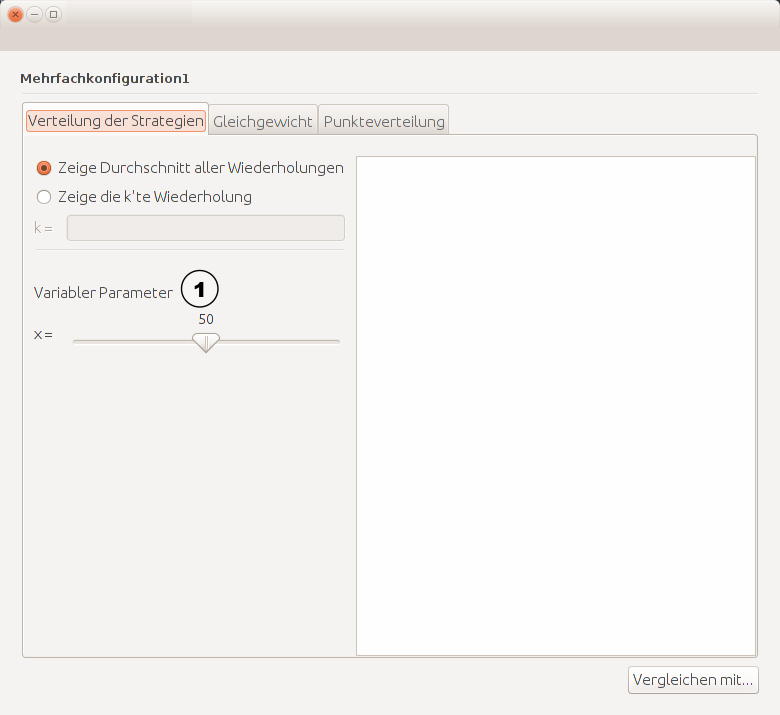
\includegraphics[width=1.1\textwidth]{GUI_Entwurf/MehrfachErgebnisse.png}
  \caption{Ergebnisfenster einer Mehrfachkonfiguration}
  \label{fig:Bild7}
\end{figure}

\begin{description}

\item[1. Variabler Parameter] Bei Ergebnissen von Mehrfachkonfigurationen, kann der variable Parameter hier verändert werden. Die Ergebnisansicht ändert sich dementsprechend.


\end{description}

\pagebreak


\subsection{Ergebnisse Vergleichen}

\begin{figure}[!hp] 
  \centering
     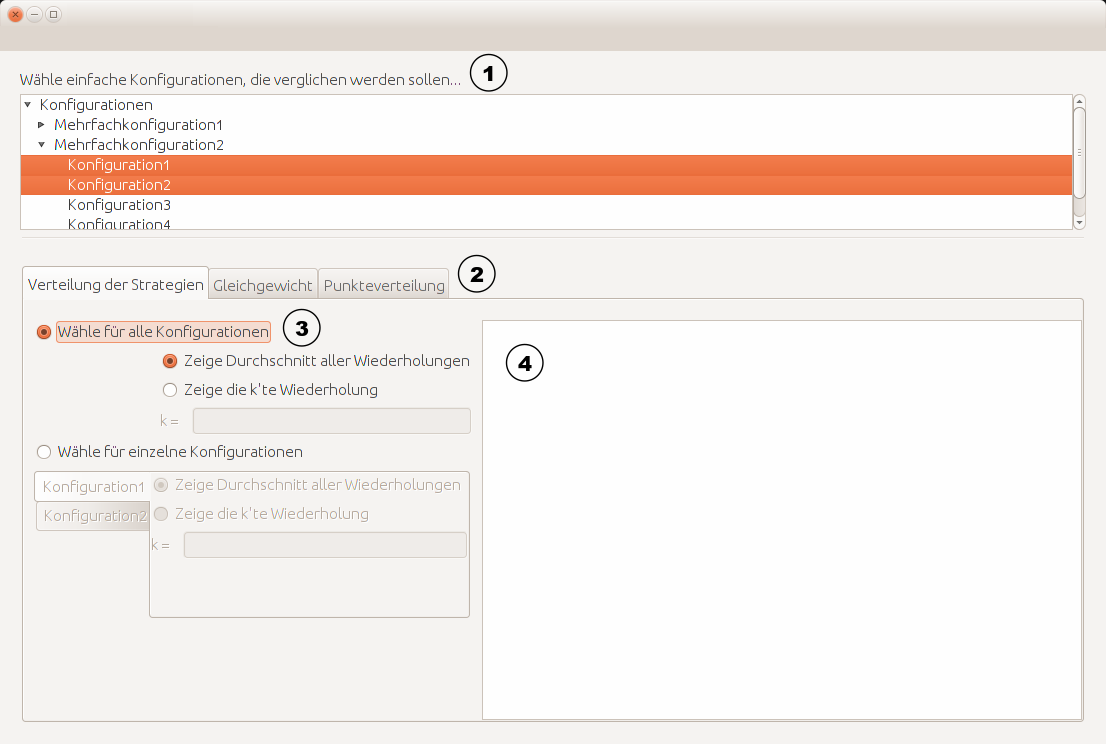
\includegraphics[width=1.15\textwidth]{GUI_Entwurf/ErgebnisseVergleichen.png}
  \caption{Vergleichenfenster}
  \label{fig:Bild1}
\end{figure}

\begin{description}

\item[1. Liste Konfigurationen] Alle Konfigurationen, zu denen Ergebnisse gespeichert wurden, werden hier angezeigt. Es können keine Mehrfachkonfigurationen ausgewählt werden. Es können mehrere Konfigurationen ausgewählt werden.

\item[2. Tabfenster] In den Tabs kann zwischen verschiedenen Ergebnissansichten gewechselt werden.

\item[3. Wiederholung] In jedem Tab kann, entweder für alle Konfigurationen oder für jede Konfihguration einzelnd, gewählt werden, ob die Ergebnisse als Durchschnitt aller Wiederholungen oder, ob die Ergebnisse einer bestimmten Wiederholung angezeigt werden sollen.

\item[4. Ergebnisfenster] In diesem Fenster werden die Ergebnisse und zugehörige Diagramme angezeigt.

\end{description}



